\section{Att multiplicera parentesuttryck}

Metoden för att lösa andragradsekvationer som presenteras ovaan fungerar för att alla $x$-termer är samlade i en kvadrat, så som $(x - 13)^2$
Tack vare det kan vi ta alla okända termer ($x$-termer) på ena sidan i en ekvation och sedan ta kvadratroten ur båda led, vilket förvandlar andragradsekvationen till (oftast) två linjära ekvationer.

Andragradsuttryck där alla okända termer är samlade i en kvadrat kallas \emph{kvadratkompletterade}, och det är inte alla gånger som andragradsuttryck är skrivna på den formen.
Vi ska lära oss att omvandla ett andragradsuttryck skrivet på allmän form ($ax^2 + bx + c$) till ett kvadratkompletterat uttryck, men innan dess måste vi bli bekväma med att multiplicera parentesuttryck som $(x+3)(2-x)$.

Hur kan man multiplicera sådana uttryck?

\subsection{Att multiplicera två parentesuttryck}

I matte 1 har vi tränat på att multiplicera parentesuttryck med ett tal.
Det gör vi genom att multiplicera \emph{varje term} i parentesen med talet framför parentesen (även kallat ``den distributiva lagen''):

\begin{center}
$7(2-x) = \framebox{7} \cdot 2 + \framebox{7} \cdot (-x) = 14 - 7x$

eller

$x(2y+x-3) = \framebox{x} \cdot 2y + \framebox{x} \cdot x + \framebox{x} \cdot (-3) = 2xy + x^2 - 3x$
\end{center}

Om vi inte har ett tal framför parentesen, utan istället ett helt parentesuttryck, kan vi göra på samma sätt:
Istället för att multiplicera varje term med $x$, multiplicerar vi med \emph{allt} som står framför parentesen.

Om vi exempelvis vill utveckla uttrycket $(x+3)(2-x)$ kan vi göra så här:

\smallskip
\begin{tabular}{l|p{5.7cm}}
  $\framebox{(x+3)} (2-x)$ & Vi ska multiplicera in $x+3$ i parentesen \\
  $= \framebox{(x+3)} \cdot 2 + \framebox{(x+3)} \cdot (-x)$ & Vi får nu två nya parentesuttryck, som vi måste utveckla vidare. Det går lättare att se vad vi gör om vi vänder på multiplikationen. \\
  $=2 \cdot \framebox{(x+3)} + (-x) \cdot \framebox{(x+3)}$ & Multiplicera in talen framför varje parentes, som vanligt. \\
  $=2 \cdot x + 2 \cdot 3 + (-x) \cdot x + (-x) \cdot 3$ & Snygga till uttrycken så att de går lättare att läsa. \\
  $=2x + 6 - x^2  - 3x$ & Förenkla uttrycket genom att slå samman $x$-termerna. (Men håll $x^2$ separat!) \\
  $=-x^2 - x + 6$ & \\
\end{tabular}
\smallskip

Den här metoden för att multiplicera parentesuttryck är bra för att den \emph{alltid} fungerar:
Om vi vill multiplicera längre uttryck eller krångligare uttryck kan vi alltid följa samma regel.
Men metoden är inte särskilt snabb, och därför kommer vi att lära oss ett par användbara genvägar.

\begin{itemize}
  \item Att \textbf{utveckla} ett uttryck är att skriva om det så att det inte är några parentesmultiplikationer kvar.
  I utvecklade uttryck är termer också sammanslagna så långt som möjligt.
  Ofta skriver man termerna med högst exponent först ($2x^2+5x-1$ istället för $5x-1+2x^2$), men det kan ibland vara snyggare att undvika att första termen är negativ ($1-2x$ istället för $-2x + 1$).
  \item Att \textbf{förenkla} ett uttryck är att skriva det på en form som går så lätt som möjligt att läsa.
  Om $(x+3)(x-2)$ eller $-x^2 - x + 6$ är lättast att läsa är en smaksak.
\end{itemize}

\subsubsection{Genväg 1: Multiplicera alla möjliga termer}

Den vanligaste genvägen för att multiplicera parentesuttryck är att ta \emph{varje} term i den ena parentesen, multiplicera med \emph{varje} term i den andra, och summera resultaten.
När man lär sig denna metod brukar man ofta rita pilar mellan termerna, så att man ser att man inte glömmer bort någon multiplikation:

\begin{figure}
  \centering
  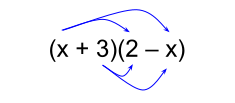
\includegraphics[width=0.7\textwidth]{bilder/parentesmultiplikation.svg}
  \caption{\label{fig:parentesmultiplikation}Utritning av pilar när man utvecklar uttrycket $(x+3)(x-2)$.}
\end{figure}

När man blivit mer van vid metoden brukar man inte rita ut pilarna längre.

Exempel: Utveckla uttrycket $(x+3)(2-x)$.

\smallskip
\begin{tabular}{l|p{5.7cm}}
  $(\framebox{x}+3)\framebox{($2-x$)}$ & Vi börjar med att multiplicera $x$ i första parentesen med varje term i andra parentesen. \\
  $= x \cdot 2 + x \cdot (-x) + (\cancel{x} + \framebox{3})\framebox{($2-x$)}$ &  Vi fortsätter med att även multiplicera trean i första parentesen. \\
  $= x \cdot 2 + x \cdot (-x) + 3 \cdot 2 + 3 \cdot (-x)$ & Multiplicera in talen framför varje parentes, som vanligt. (Alla termer är nu multiplicerade.) \\
  $= 2x - x^2 + 6 - 3x$ & Förenkla uttrycket genom att slå samman $x$-termerna. \\
  $=-x^2 - x + 6$ & \\
\end{tabular}
\smallskip

Ett sätt att motivera varför den här metoden fungerar är att rita upp multiplikationen som en areaberäkning.

(To be written)

\subsubsection{Genväg 2: Kvadreringsreglerna $(a+b)^2$ och $(a-b)^2$}

När man multiplicerar parentesuttryck som är kvadrater kan man använda en särskild genväg, som kallas \emph{kvadreringsreglerna}.

(To be written)

\subsubsection{Genväg 3: Konjugatregeln $(a+b)(a-b)$}

(To be written)

\subsection{Fördjupning: Att multiplicera fler än två parentesuttryck}

Hittills har vi tittat på hur man multiplicerar två parentesuttryck.
Men vad händer om vi skulle ha fler parenteser?
Hur utvecklar vi ett uttryck som $(x+1)(5-2x)(y+x)$?

Det finns flera sätt att hantera dessa multiplikationer, och en metod som alltid fungerar är denna:
Multiplicera två delar i taget, och fortsätt tills alla parenteser är utvecklade.

Vad betyder det?
Jo, istället för att se det som \emph{tre} uttryck som ska multipliceras, kan du se det som att du multiplicerar två parenteser och \emph{sedan} multiplicerar med det tredje:

\smallskip
\begin{tabular}{l|p{5.7cm}}
  $(x+1)(5-2x)(y+x)$ & Välj två av parenteserna, och börja med att multiplicera dem. \\
  $= \framebox{$(x+1)(5-2x)$} \cdot (y+x)$ & Använd den metod du tycker fungerar bäst för att multiplicera. \\
  $= \framebox{$(-2x^2 + 3x + 5)$} \cdot (x+y) $ & Fortsätt sedan genom att multiplicera med nästa parentes. \\
  $= \ldots & (Använd den metod du tycker fungerar bäst.) \\
  $= -2x^3 - 2x^2y + 3xy + 5y$
\end{tabular}
\smallskip

\subsection{Uppgifter}

(Endast skisser!)

\begin{enumerate}
  \item Använd den associativa lagen för att multiplicera parentesuttryck för att utveckla de här uttrycken:
  \begin{enumerate}[a)]
    \item $(x+3)(x+4)$
    \item $(2a-1)(1-a)$
    \item $(0{,}5t+1)(0{,}5t-1)$
  \end{enumerate}
  \item Använd metoden med att multiplicera varje term för att utveckla de här uttrycken:
  \begin{enumerate}[a)]
    \item $(3+x)(2x+4)$
    \item $(a-2)(1-2a)$
    \item $(0{,}5s+10)(0{,}5s-10)$
  \end{enumerate}
  \item Vilka av de här uttrycken kan man använda kvadrerings- eller konjugatreglerna för att utveckla?
  \begin{enumerate}[a)]
    \item $(7x+2)(3{,}5x+1)$
    \item $(p+1)(p+1)$
    \item $(20+x)(x-20)$
    \item \ldots
  \end{enumerate}
  \item Utveckla några av dessa uttryck med kvadrerings- eller konjugatreglerna, och andra med en annan metod.
  Ta tid på hur lång tid det tar, och räkna ut hur många procent snabbare det går med kvadrerings- eller konjugatreglerna.
  \begin{enumerate}[i)]
    \item \ldots
  \end{enumerate}
  \begin{enumerate}[a)]
    \item Hur lång tid tog det att utveckla ett uttryck med kvadrerings- eller konjugatreglerna, i genomsnitt?
    \item Hur lång tid tog det att utveckla ett uttryck med någon annan metod, i genomsnitt?
    \item Hur mycket snabbare/långsammare är kvadrerings- eller konjugatreglerna, i genomsnitt?
  \end{enumerate}
  \item Med hjälp av konjugatregeln kan man i huvudet beräkna multiplikationen $102 \cdot 98$.
  \begin{enumerate}[a)]
    \item Kan du se hur konjugatregeln kan vara till nytta?
    \item Vad blir $102 \cdot 98$?
    \item Kan du ge exempel på någon annan multiplikation där man kan använda konjugatregeln för huvudräkning?
  \end{enumerate}
  \item \ldots
  
\end{enumerate}

(To be written)
